\subsection{Hasil dan Perbandingan dengan \textit{Scikit-learn}}
\label{subsec:lr-hasil}

Implementasi \textit{from scratch} dibandingkan dengan kelas \texttt{LogisticRegression} dari \texttt{sklearn.linear\_model} \cite{pedregosa2011sklearn,sklearn-lr-guide} untuk setiap jenis penalti. Setiap penalti diwakili oleh konfigurasi terbaiknya menurut validasi silang (Tabel~\ref{tab:lr-cv}); keempatnya memakai \textit{solver} IRLS-CD pada implementasi \textit{scratch}. Agar perbedaan hanya berasal dari implementasi, kedua model memakai \textit{preprocessing}, \texttt{train\_set} (21.847 baris), dan \texttt{val\_set} (5.462 baris) yang sama, dengan \textit{threshold} 0,5. Kedua implementasi meminimumkan fungsi tujuan yang setara. \texttt{lr.py} meminimumkan rata-rata \textit{log-loss} ditambah $\lambda\,\Omega(w)$, sedangkan \textit{scikit-learn} meminimumkan $C\sum_i \text{log-loss}_i + \Omega(w)$, sehingga $C = 1/(n\lambda)$ dan \texttt{l1\_ratio} $=\rho$. \textit{Scikit-learn} memakai \texttt{lbfgs} untuk tanpa penalti dan L2, serta \texttt{saga} untuk L1 dan \textit{Elastic Net} (\texttt{lbfgs} tidak mendukung penalti L1), dengan \texttt{tol} $10^{-6}$ dan maksimum 5.000 iterasi.

\begin{table}[H]
	\centering
	\caption{Perbandingan LR \textit{from scratch} dan \textit{scikit-learn} pada \texttt{val\_set} (\textit{threshold} 0,5). \textit{Precision} dan \textit{recall} untuk kelas batal. Waktu adalah waktu pelatihan satu model pada \texttt{train\_set} di komputer yang dipakai (nilai kasar, lihat analisis).}
	\label{tab:lr-hasil}
	\small
	\resizebox{\textwidth}{!}{%
	\begin{tabular}{l c c c c c c c}
		\toprule
		\textbf{Implementasi} & \textbf{Macro F1} & \textbf{Acc.} & \textbf{Prec.} & \textbf{Recall} & \textbf{ROC-AUC} & \textbf{Waktu (s)} & \textbf{Bobot 0} \\
		\midrule
		\textit{Scratch} -- Tanpa penalti & 0,7731 & 0,8067 & 0,7333 & 0,6439 & 0,8735 & 7,5 & 2 \\
		\textit{Sklearn} -- Tanpa penalti & 0,7731 & 0,8067 & 0,7333 & 0,6439 & 0,8736 & 35,8 & 2 \\
		\midrule
		\textit{Scratch} -- L1 & 0,7739 & 0,8072 & 0,7335 & 0,6462 & 0,8741 & 9,2 & 16 \\
		\textit{Sklearn} -- L1 & 0,7736 & 0,8070 & 0,7333 & 0,6456 & 0,8741 & 362,3 & 14 \\
		\midrule
		\textit{Scratch} -- L2 & 0,7720 & 0,8057 & 0,7316 & 0,6428 & 0,8739 & 13,1 & 2 \\
		\textit{Sklearn} -- L2 & 0,7720 & 0,8057 & 0,7316 & 0,6428 & 0,8739 & 2,2 & 2 \\
		\midrule
		\textit{Scratch} -- \textit{Elastic Net} & 0,7722 & 0,8059 & 0,7320 & 0,6428 & 0,8740 & 10,9 & 13 \\
		\textit{Sklearn} -- \textit{Elastic Net} & 0,7722 & 0,8059 & 0,7320 & 0,6428 & 0,8740 & 382,9 & 12 \\
		\bottomrule
	\end{tabular}}
\end{table}

Konfigurasi yang dibandingkan adalah tanpa penalti, L1 ($\lambda = 10^{-4}$), L2 ($\lambda = 10^{-4}$), dan \textit{Elastic Net} ($\lambda = 10^{-4}$, $\rho = 0{,}5$). Kolom ``Bobot 0'' menghitung bobot yang tepat nol dari 100 bobot. Kedua kolom pada baris tanpa penalti dan L2 bernilai 2 karena dua kolom fitur interaksi (\texttt{lead\_bin3\_x\_\allowbreak Airline} dan \texttt{lead\_bin4\_x\_\allowbreak Airline}) selalu bernilai nol, bukan karena regularisasi (Subbab~\ref{subsec:lr-implementasi}).

\begin{figure}[H]
	\centering
	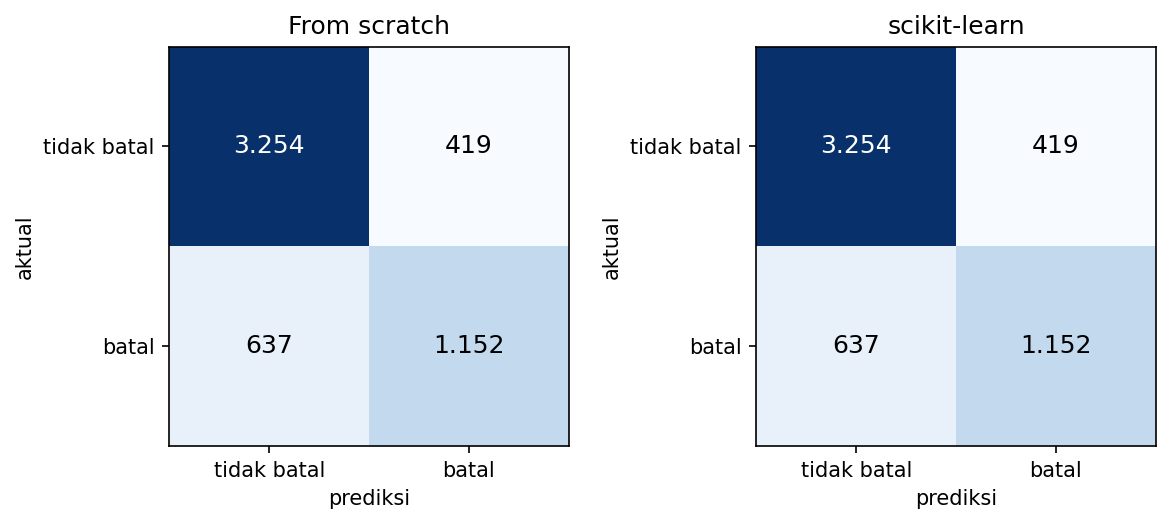
\includegraphics[width=0.8\textwidth]{lr/lr_confusion_matrix.png}
	\caption{\textit{Confusion matrix} LR tanpa penalti (konfigurasi terbaik) pada \texttt{val\_set}, \textit{from scratch} (kiri) dan \textit{scikit-learn} (kanan)}
	\label{fig:lr-cm}
\end{figure}

\subsubsection{Kurva \textit{Loss}}
Gambar~\ref{fig:lr-loss} memperlihatkan nilai fungsi tujuan $J$ (\textit{log-loss} ditambah penalti) pada \texttt{train\_set} untuk setiap penalti, dengan kedua \textit{solver} yang diimplementasikan. Nilai $J$ tidak dapat dibandingkan langsung antarpenalti karena suku penaltinya berbeda; yang dibandingkan adalah bentuk konvergensinya.

\begin{figure}[H]
	\centering
	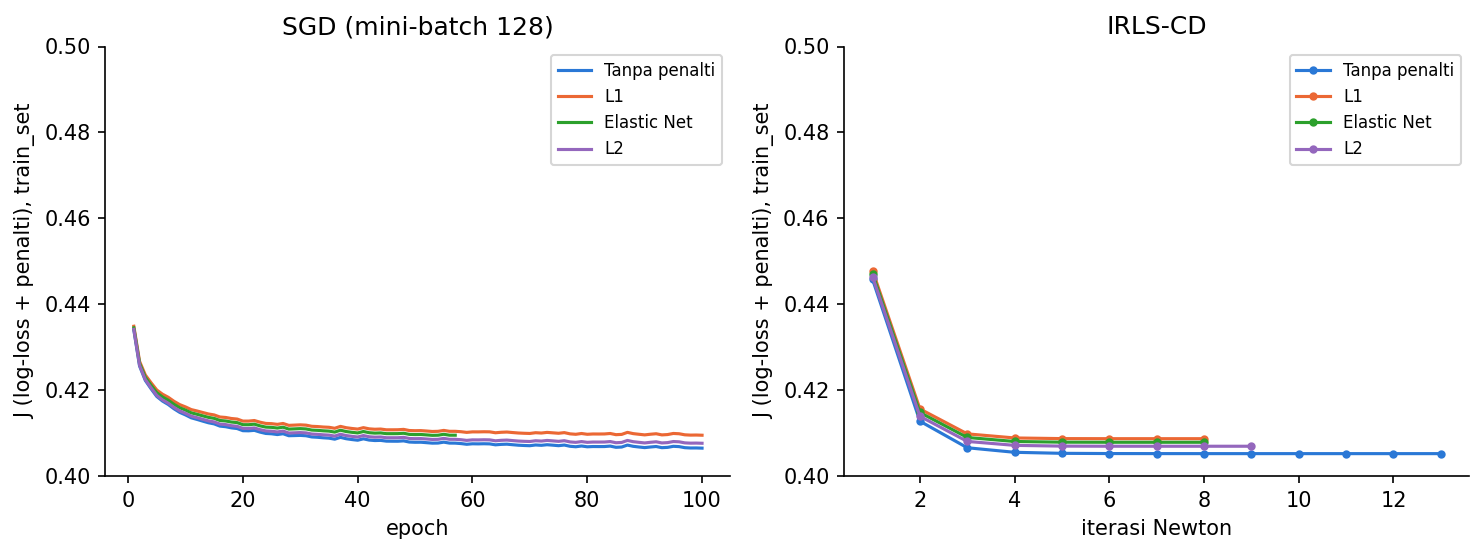
\includegraphics[width=\textwidth]{lr/lr_loss_curves.png}
	\caption{Kurva $J$ per iterasi pada \texttt{train\_set}: SGD \textit{mini-batch} per \textit{epoch} (kiri) dan IRLS-CD per iterasi Newton (kanan)}
	\label{fig:lr-loss}
\end{figure}

\begin{itemize}
	\item \textbf{SGD} menurun cepat pada sekitar 10 \textit{epoch} pertama, lalu melandai dan masih turun perlahan saat berhenti. Tiga dari empat konfigurasi berhenti di batas 100 \textit{epoch}; hanya \textit{Elastic Net} berhenti lebih awal (57 \textit{epoch}) karena perubahan \textit{loss} di bawah toleransi. Kurvanya sedikit bergerigi karena gradien \textit{mini-batch} bersifat acak, dan \textit{learning rate} yang tetap membuatnya tidak pernah menetap di satu titik. Ini berarti SGD belum benar-benar konvergen pada 100 \textit{epoch}.
	\item \textbf{IRLS-CD} mencapai nilai akhirnya dalam 8 sampai 13 iterasi. Pada tanpa penalti dibutuhkan 13 iterasi, lebih banyak daripada penalti lain (8 sampai 9), karena tidak ada suku penalti yang membuat masalah lebih terkondisi dengan baik; model ini juga memiliki kolom yang kolinear (Subbab~\ref{subsec:lr-implementasi}).
	\item Untuk setiap penalti, $J$ akhir IRLS-CD lebih rendah daripada SGD: 0,4052 terhadap 0,4065 (tanpa penalti), 0,4087 terhadap 0,4095 (L1), 0,4079 terhadap 0,4095 (\textit{Elastic Net}), dan 0,4070 terhadap 0,4076 (L2). Karena fungsi tujuannya konveks, selisih ini adalah jarak SGD ke optimum, yang menjelaskan mengapa IRLS-CD sedikit lebih baik pada validasi (Subbab~\ref{subsubsec:lr-optimasi}).
\end{itemize}

\subsubsection{Analisis}
\paragraph{Hasil praktis identik.} Untuk keempat penalti, selisih Macro F1 antara \textit{scratch} dan \textit{scikit-learn} paling besar 0,0003 (L1), ROC-AUC berselisih paling besar $10^{-4}$, dan matriks konfusinya sama persis atau berbeda satu baris. Label prediksi sama pada 99,98\% sampai 100\% baris, dan korelasi peluang model terbaik 1,0000. Ini sesuai harapan: keduanya meminimumkan fungsi tujuan konveks yang sama, sehingga IRLS-CD dan \textit{solver} \textit{scikit-learn} menuju optimum yang sama. Perbedaan kecil pada L1 berasal dari kriteria berhenti yang berbeda: \texttt{saga} berhenti pada toleransi tertentu dan belum tentu tepat di optimum, sedangkan IRLS-CD pada L1 menghasilkan nilai $J$ sedikit lebih rendah (0,408706 terhadap 0,408709).

\paragraph{Bobot dan \textit{sparsity}.} Selisih bobot terbesar (nilai mutlak) antara kedua implementasi adalah 5,85 (tanpa penalti), 0,100 (L1), 0,062 (\textit{Elastic Net}), dan 0,0028 (L2). Selisih besar pada model tanpa penalti bukan tanda kesalahan. Kolom \textit{one-hot} setiap fitur kategorikal bersama bias saling kolinear (matriks fitur ditambah bias hanya berperingkat 92 dari 101), sehingga bobotnya tidak unik walaupun prediksinya identik (label sama 100\%). Penalti L2 memperbaiki hal ini karena menjamin solusi yang unik, dan itu terlihat dari selisih bobotnya yang sangat kecil. Pada L1 dan \textit{Elastic Net}, kedua implementasi menghasilkan bobot tepat nol dalam jumlah hampir sama (16 terhadap 14 dan 13 terhadap 12). Selisih satu sampai dua bobot muncul karena bobot-bobot itu berada tepat di dekat ambang \textit{soft-thresholding}, dan kriteria berhenti kedua \textit{solver} berbeda.

\paragraph{Waktu pelatihan.} Waktu pada Tabel~\ref{tab:lr-hasil} hanya perkiraan kasar karena diukur sekali pada komputer yang sedang dipakai untuk pekerjaan lain. Pengulangan pengukuran yang sama memberi angka yang berbeda beberapa kali lipat (misalnya \textit{scikit-learn} tanpa penalti: 10,9 detik pada satu kali jalan dan 35,8 detik pada kali lain), sehingga hanya selisih yang besar yang bermakna. Terlihat dua pola. \textit{Scikit-learn} jauh lebih cepat pada L2 (2,2 terhadap 13,1 detik), karena \texttt{lbfgs} yang ditulis dalam kode teroptimasi hanya perlu menghitung gradien, sedangkan IRLS-CD membentuk dan memperbarui matriks Gram $101 \times 101$ pada setiap iterasi. Sebaliknya \textit{scratch} jauh lebih cepat pada L1 dan \textit{Elastic Net} (sekitar 9 sampai 11 detik terhadap lebih dari 360 detik), karena \texttt{saga} adalah metode orde pertama yang butuh banyak lintasan data sampai mencapai toleransi $10^{-6}$ pada fitur yang berkorelasi, sedangkan IRLS-CD memakai informasi orde kedua dan konvergen dalam kurang dari sepuluh iterasi. Pada model tanpa penalti \textit{scratch} juga lebih cepat (7,5 terhadap 35,8 detik), tetapi selisih ini paling tidak stabil antarpengukuran. Perbandingan ini adil hanya dalam arti kedua \textit{solver} diminta ketat pada toleransi masing-masing; \textit{scikit-learn} dapat dipercepat dengan toleransi yang lebih longgar tanpa mengubah hasil prediksi secara berarti.

\paragraph{Keterbatasan.} (i) Perbandingan dilakukan pada satu pembagian \texttt{train\_set}/\allowbreak\texttt{val\_set}, dan \texttt{val\_set} ikut dipakai dalam CV sehingga bukan estimasi independen (Subbab~\ref{subsec:lr-validasi}). (ii) Selisih antarpenalti (paling besar 0,002 pada Macro F1) jauh di bawah simpangan baku antar-\textit{fold} (0,0073), sehingga urutan penalti pada tabel tidak bermakna secara statistik. (iii) Seluruh hasil \textit{scratch} di atas memakai IRLS-CD. Hasil \textit{scratch} dengan \textit{solver} SGD yang sesuai materi kelas sedikit di bawahnya (Subbab~\ref{subsubsec:lr-optimasi}); karena SGD belum konvergen, selisihnya dengan \textit{scikit-learn} akan lebih besar dari angka di atas.
